\section[Target (C. Keith)]{Target \label{sec:target} }
A schematic diagram of the GlueX cryotarget is shown in Fig.~\ref{fig:Target}.  
The major components of the system are a pulse tube cryocooler,\footnote{Cryomech model PT415.}
a condenser, and a target cell.  These items are contained within
an aluminum and stainless steel `L'-shaped vacuum chamber
with an extension of closed-cell foam\footnote{Rohacell 110XT, Evonik Industries AG.}
surrounding the target cell.
In turn, the GlueX start counter (Sec.~\ref{sec:st}) surrounds the
foam chamber and is supported by the horizontal portion of the vacuum chamber.
Polyimide foils, 100$\mu$m thick, are used at the upstream and downstream ends of the
chamber as beam entrance and exit windows.
The entire system, including the control electronics, vacuum pumps,
gas-handling system, and tanks for hydrogen
storage, are mounted on a small cart that is attached to a set of rails for
insertion into the GlueX solenoid.  To satisfy the laboratory's flammable gas safety requirements,
the system is connected at multiple points to a nitrogen-purged ventilation pipe that
extends outside Hall D. 
\begin{figure*}
\begin{center}
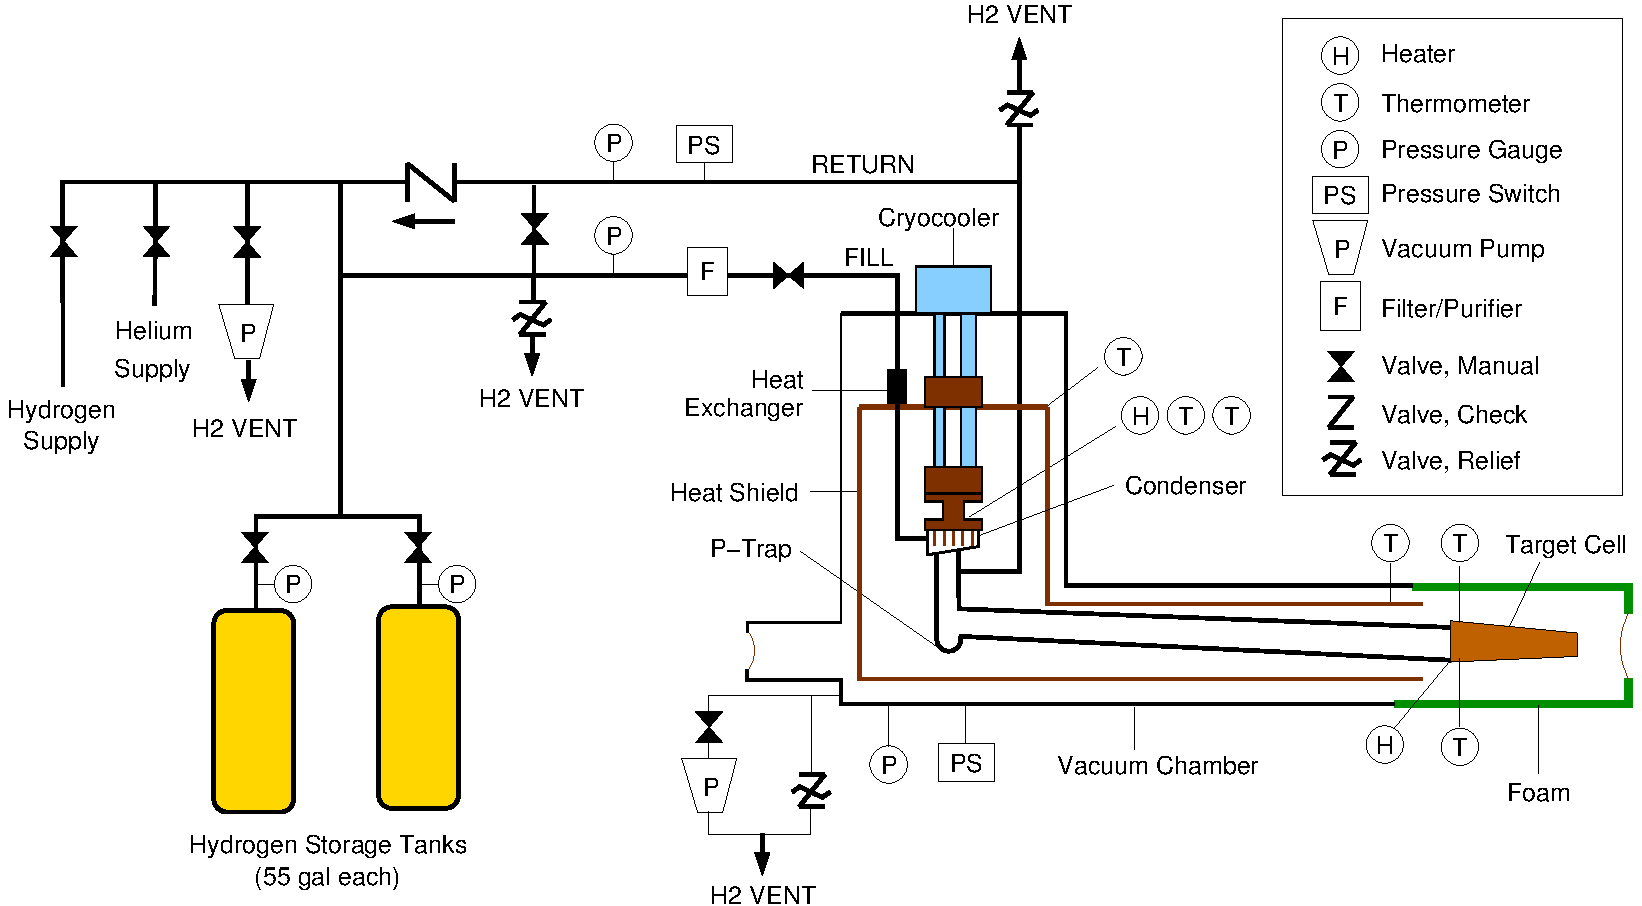
\includegraphics[width=5in]{figures/TargetSchematic2.pdf}
\end{center}
\caption{Simplified process and instrumentation diagram for the GlueX liquid hydrogen target (not to scale).
In the real system, the P-trap is above the level of the target cell and is used to
promote convective cooling of the target cell from room temperature.}
\label{fig:Target}
\end{figure*}

Hydrogen gas is stored inside two 200~l tanks and
is cooled and condensed into a small copper and stainless steel container,
the condenser, that is thermally anchored to the second cooling stage of the cryocooler. 
The first stage of the cryocooler is used to
cool the H$_2$ gas to about 50~K before it enters the condenser.
It also cools a copper thermal shield that surrounds all
lower temperature components of the system except for the
target cell itself, which is wrapped in a few layers of aluminized-mylar/cerex insulation.

The condenser is comprised of a copper C101 base
sealed to a stainless steel can with an indium o-ring.  Numerous vertical 
fins are cut into the copper base, giving a large surface area for condensing hydrogen gas.
A heater and a pair of calibrated cernox thermometers\footnote{Lake Shore Cryotronics.}
are attached outside the condenser and are used to regulate its temperature when the
system is filled with liquid hydrogen.

The target cell, shown in Fig.~\ref{fig:TargetCell}, is similar to
designs utilized in Hall B at Jefferson Lab for many years~\cite{HAKOBYAN2008218}.  
The cell walls are made from 100~$\mu$m thick aluminized
polyimide sheet that is wrapped in a conical shape and glued along the edge,
overlapping in a 2~mm wide scarf joint.  
The conical shape prevents bubbles from collecting inside the cell, while the
scarf joint reduces the stress riser at the glue joint.  This conical
tube is glued to an aluminum base 
along with stainless steel fill and return tubes leading to the condenser, a feed-thru for two
calibrated cernox thermometers inside the cell, and a
polyamide-imide support for the reentrant, upstream beam window.  
Both the upstream and downstream beam
windows are made of non-aluminized,
100~$\mu$m thick polyimide films that have been extruded into the
shapes indicated in Fig.~\ref{fig:TargetCell}. All items are glued together using
a two-part epoxy\footnote{3M Scotch-Weld epoxy adhesive DP190 Gray.}
that has been in reliable use at cryogenic temperatures at
Jefferson Lab for many years. 
A second  heater is attached to the aluminum base and
is used to boil the liquid from the cell for empty target measurements.
The base is attached to a kinematic mount which is in turn
supported inside the vacuum chamber using a system of carbon fiber rods.    
The mount is used to correct the pitch and yaw
of the cell, while $x$, $y$, and $z$ adjustment 
is accomplished using positioning screws on the target cart. 


During normal operation sufficient hydrogen gas is condensed from the storage tanks
until the target cell, condenser, and interconnecting piping are filled with liquid hydrogen
and an equilibrium pressure of about 20~psia is achieved.  
The condenser temperature is regulated at 18~K, while the
liquid in the cell cools to about 19.8~K.  This is 1.5~K below the saturation
temperature of H$_2$ and eliminates boiling within the cell, thus permitting a more
accurate determination of the fluid density.  
The system can be cooled from room temperature and filled with liquid hydrogen in
about six hours.
For empty target runs, the liquid in the system is boiled back into the storage tanks using the heater
attached to the cell's aluminum base, which takes about five minutes.  During this
mode of operation, H$_2$ gas continues to condense and drain towards the target cell, where it
is evaporated by the cell heater.  In this way, the cell does not warm above 40~K, and
it can be re-filled with liquid hydrogen in about twenty minutes.

\begin{figure}
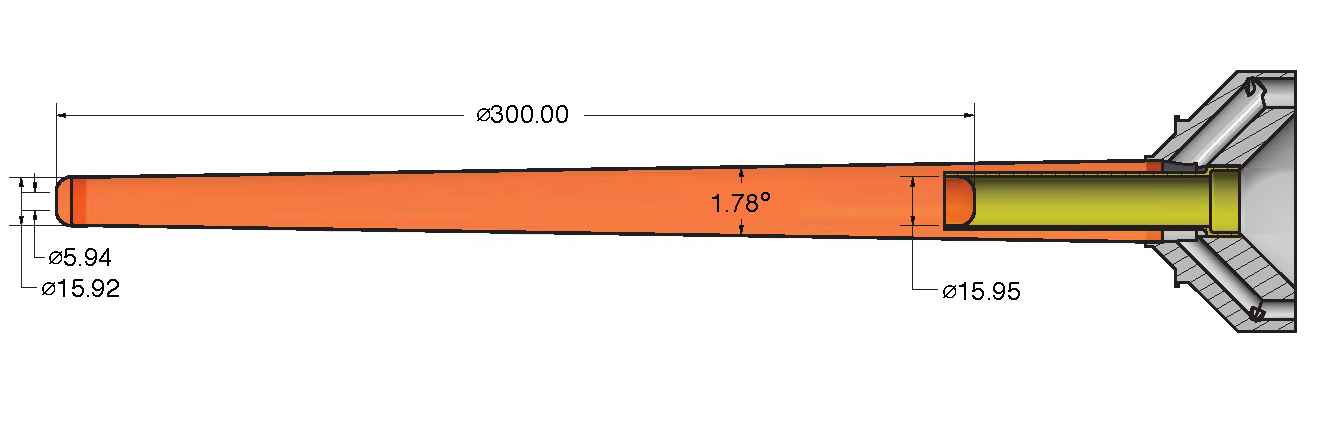
\includegraphics[width=3.5in]{figures/GluexCell_mm.pdf}
\caption{Target cell for the liquid hydrogen target.  Dimensions are in mm.  The photon beam
tranverses the target right to left in this drawing.}
\label{fig:TargetCell}
\end{figure}

The cryotarget is controlled using a
National Instruments CompactRIO 9030, which is an industrial embedded controller 
capable of running LabVIEW programs on top of an AMD64 Linux environment. 
Control logic and equipment interface is handled by a LabVIEW program, 
while a standard EPICS softIOC running in Linux provides a
bridge between the controller and JLab's EPICS enviroment. The LabVIEW program interacts
with the softIOC using National Instrument's DSC module.    
Temperature read back and control of the condenser and target cell thermometers
are managed by a four-input temperature
controller with PID control loops of 50 and 100~W\footnote{Lake Shore Model 336.}.
Strain gauge pressure sensors measure the fill and return pressures with 0.25\% 
accuracy.  

Operation of the cryotarget is highly automated and requires minimal user intervention.
Most tasks can be performed by pressing one of two main buttons on
the Graphical User Interface: {\bf Fill Target} and {\bf Empty Target}.
Each button checks the status of the cryocooler, hydrogen gas pressure, insulating vacuum, etc.\
and loads appropriate settings for alarm values and temperature-control set points.  
When the expected equilibrium readings for a full (or empty) target are achieved, the
GUI informs the user that the target is stable and ready for beam.  A third button, {\bf Target Off},
simply turns off the cryocooler and allows the system to warm over the course of a few days.

The GlueX cryotarget has operated in a very reliable and predictable manner throughout the
experiment.  When filled with subcooled liquid, its long-term temperature ($\pm 0.2$~K) and
and pressure ($\pm 0.1$~psi) stability enable a determination of the liquid density to better than 0.5\%.
It has also demonstrated the capability to condense helium
in the target cell and operate in a stable manner at 4.2~K.  However, this requires extending the
thermal shield to surround the target cell. A thin (1~mm) aluminum shell, clamped to the end
of the existing copper shield is sufficient for this purpose.
